\documentclass{kththesis}

\usepackage{blindtext} % This is just to get some nonsense text in this template, can be safely removed

\usepackage{csquotes} % Recommended by biblatex
\usepackage{biblatex}
\usepackage{mathtools}
\usepackage{caption}
\usepackage{subcaption}
\usepackage{enumerate}
\usepackage{gensymb}
\usepackage{multirow}
\usepackage{float}
\usepackage{amsmath,amssymb}
\usepackage{listings}

\DeclareRobustCommand{\bbone}{\text{\usefont{U}{bbold}{m}{n}1}}

\DeclareMathOperator{\EX}{\mathbb{E}}
\DeclareMathOperator{\Lagr}{\mathcal{L}}

\addbibresource{ex.bib} % The file containing our references, in BibTeX format


\title{Investigation of deep learning approaches for overhead imagery analysis}
\alttitle{Utredning av djupinlärnings metoder för satellit och flygbilder}
\author{Joar Gruneau}
\email{joarg@kth.se}
\supervisor{Kevin Smith}
\examiner{Danica Kragic}
\programme{Master in Computer Science}
\school{School of Electrical Engineering and Computer Science}
\date{\today}


\begin{document}

% Frontmatter includes the titlepage, abstracts and table-of-contents
\frontmatter

\titlepage

\begin{abstract}
Analysis of overhead imagery has a great potential to produce real time data cost effectively. This can be an important foundation for decision-making for businesses and politics. Every day a massive amount of new satellite imagery is produced. To fully take advantage of these data volumes a computationally efficient pipeline is required for the analysis. This thesis proposes a pipeline which outperforms the Segment Before you Detect network \parencite{audebert_usability_2016} and different types of fast region based convolutional neural networks \parencite{zhong_robust_2017-1} with a large margin in a fraction of the time. The model obtains a prediction error for counting cars of 1.67\% on the Potsdam dataset and increases the vehicle wise F1 score on the Vedai dataset from 0.305 reported by \parencite{zhong_robust_2017-1} to 0.542. This thesis also shows that it is possible to outperform the  Segment Before you Detect network in less than 1\% of the time on car counting and vehicle detection while also using less than half of the resolution. This makes the proposed model a viable solution for large scale satellite imagery analysis.
\end{abstract}


\begin{otherlanguage}{swedish}
  \begin{abstract}
Analys av flyg och satellit bilder har stor potential att kostnadseffektivt producera data i realtid  för beslutsfattande för företag och politik. Varje dag produceras massiva mängder nya satellitbilder. För att fullt kunna utnyttja dessa datamängder krävs en beräkningseffektivt nätverk för analysen. Denna avhandling föreslår ett nätverk som överträffar Segmentet Before you Detect nätverket  \parencite{audebert_usability_2016} och olika typer av snabbt regionsbaserade convolutional neurala nätverk \parencite{zhong_robust_2017-1} med en stor marginal på en bråkdel av tiden. Den föreslagna modellen erhåller ett prediktionsfel för att räkna bilar på 1,67\% på Potsdam datasetet och ökar F1-poängen for fordons detektion på Vedai datasetet från 0.305 rapporterat av \parencite{zhong_robust_2017-1} till 0.542. Denna avhandling visar också att det är möjligt att överträffa Segment Before you Detect nätverket på mindre än 1 \% av tiden på bilräkning och fordonsdetektering samtidigt som den föreslagna modellen använder mindre än hälften av upplösningen. Detta gör den föreslagna modellen till en attraktiv lösning för storskalig satellitbildanalys.
  \end{abstract}
\end{otherlanguage}


\tableofcontents


% Mainmatter is where the actual contents of the thesis goes
\mainmatter


\chapter{Introduction}
Convolutional neural networks (CNN) have had great success for computer vision tasks \parencite{sermanet_overfeat:_2013,zeiler_visualizing_2013,  simonyan_two-stream_2014, krizhevsky_imagenet_2012}.
The success is possible in part thanks to graphical processing units (GPUs) and large scale human annotated datasets which  the networks can learn from. CNN have progressed from single object detection in images \parencite{krizhevsky_learning_2009} to multiple object detection and bounding box prediction \parencite{lin_microsoft_2014}. CNN networks have also had great success in different segmentation task \parencite{garcia-garcia_review_2017}. There is a similar trend in segmentation where we are moving from the easier task of semantic segmentation to the more complex task of instance segmentation. In semantic segmentation every pixel is mapped to a class and in instance segmentation the different instances of objects are separated detected for each class. It is not trivial to construct a loss function for segmentation which enforces the desired properties into the segmentation network. Much work has gone into this problem which has resulted in several different types of loss functions \parencite{ronneberger_u-net:_2015, yu_unitbox:_2016, rahman_optimizing_2016}. Often the loss function fails to enforce important properties such as spatial contiguity in the segmentation maps \parencite{luc_semantic_2016} or proper spatial separation of objects \parencite{audebert_segment-before-detect:_2017}. Conditional Markov random fields (CRFs) have been a popular post processing step to ensure spatial contiguity in segmentation maps \parencite{zhao_classification_2007}. Ronneberger \textit{et al.} \parencite{ronneberger_u-net:_2015} also shows that object separation can be enforced by weighting the pixel wise loss function based on the proximity to nearby objects.\\
\\
A new popular network for image to image translations are generative adversarial networks. The network consists of a generator network which performs the image translation and a discriminative network which aims to learn the loss function to differentiate the generated samples from the ground truth ones \parencite{goodfellow_nips_2016}. These type of networks have had great success on image to image translation tasks and are able to produce much more artistically pleasing mappings then networks without the adversarial loss \parencite{ledig_photo-realistic_2016, isola_image--image_2016}. The success comes from the general approach where the network can learn its own loss function which has proven beneficial for many tasks where a effective loss function is hard to express. These types of networks have also been applied to image segmentation and has shown to give an increased performance \parencite{luc_semantic_2016, souly_semi_2017}. GANs have proven to be especially successful on small dataset such as medical segmentation where the human annotations usually are costly due to the required medical expertise needed to create correct annotations \parencite{souly_semi_2017, xue_segan:_2017, yang_automatic_2017, rezaei_conditional_2017, arbelle_microscopy_2017}.\\
\\
\\
In today's information society data is becoming more and more valuable. The data is used as a foundation to do business decisions  as well as political decisions daily. The life time of new data is also decreasing and new data is considered old and unrepresentative much faster than before. Thanks to the large number of satellites and the low cost to produce high resolution satellite images, analysis of satellite images can be a useful tool to obtain real time data cost effectively. To mention a few applications it can be used for traffic flow monitoring \parencite{ruhe_traffic_2003, moranduzzo_automatic_2014} vegetation monitoring \parencite{uto_characterization_2013, berni_thermal_2009}, urban area monitoring \parencite{moranduzzo_lbp-based_2015}, water reserve capacity monitoring, generating new maps \parencite{isola_image--image_2016} and even to detect endangered whales \parencite{polzounov_right_2016}. Investors are continuously competing to obtain an edge over their competitors and turn a profit. Here satellite imagery analysis can be used to obtain fresh information before it reaches the market. For example, if we continuously can count the number of vehicles outside a marketplace we can more accurately predict how many customers that are visiting the marketplace and therefore make more accurate predictions about the markets earnings before those earnings are released to the public market.\\
\\
Much research has been performed investigating object detection and more specifically vehicle detection in overhead imagery \parencite{ammour_deep_2017, holt_object-based_2009, audebert_segment-before-detect:_2017, razakarivony_vehicle_2015, zhong_robust_2017, audebert_usability_2016, sakla_deep_2017}. However object detection in overhead images has proven to be a troublesome area. The objects of interest are usually very small compared to the image and there can be multiple objects within image. This causes naive classification networks to achieve bad performance if the entire image is fed in at once \parencite{ammour_deep_2017}. To combat this some form of segmentation is usually done and the image is fed into the network in patches. Earlier methods fed explicit image patches through the CNN using sliding window techniques\parencite{holt_object-based_2009}. This achieved good performance but at a great computational cost since redundant computation of low-level filters for overlapping patches had to be performed \parencite{luc_semantic_2016}. To combat this different forms of segmentation algorithms were used such as the mean-shift-algorithm which drastically decreased the number of patches which had to be fed through the network \parencite{ammour_deep_2017}. \\
\\
This thesis investigate how to define a loss function which enforces good vehicles separation directly into the segmentation network for overhead imagery. Two different approaches are investigated, weighting the loss based on vehicle separation and adding an adversarial loss term. In both cases the desired outcome is to force the network to pay closer attention to segmentation around nearby objects. The different instances of vehicles can then be extracted directly from the segmentation maps by connected component extraction. This pipeline would achieve superior speed compared to earlier more modern methods which usually uses a two stage approach since only a single stage network would be needed at training and testing.\\
\\
An example of these types of two stage detection networks is the Segment Before You Detect (SBD) \parencite{audebert_segment-before-detect:_2017} and the fast region-based convolutional network (fast R-CNN) \parencite{ren_faster_2015, girshick_fast_2015} or mask region-based convolutional network (mask R-CNN). The SBD pipeline uses a segmentation network to find the vehicle patches. The patches are then extracted and fed into a classification network to predict vehicles and find bounding boxes. The fast R-CNN or mask R-CNN \parencite{he_mask_2017} achieves superior speed compared to the SBD pipeline. These networks uses a second stage region proposal network (RPN) to compute the bounding box predictions on internal convolutional feature maps. This approach minimizes computational time since layers can be shared. However these networks can only predict some predefined ratio of bounding boxes and the two stage network adds complexity both at training and test time.
\section{Research Question}
In this thesis we will investigate if it is possible to construct a loss function which enforces vehicle separation directly into the segmentation network for satellite imagery. The goal is to enforce  good enough vehicle separation so instances of vehicles can be directly found by connected component extraction in the segmentation map. The proposed models will be compared to the network trained with the standard cross entropy loss to measure improvements. The metrics for evaluation will be pixel wise F1 score and vehicle wise F1 score as well as visual inspection of the segmentation maps. The final model will be compared with earlier work such as the SBD and fast R-CNN on the Potsdam and Vedai datasets on the metrics pixel wise F1 score, vehicle wise F1 score, prediction error counting cars and evaluation time.
\chapter{Background}
\section{Generative adversarial networks}
Goodfellow \textit{et al.} \parencite{goodfellow_nips_2016} first proposed the generative adversarial network (GAN). The network consists of two parts, a generator and a discriminator. The generator's task is to generate samples from some data distribution. The discriminators task is to differentiate these generated samples from the true samples. This results in a counter fitting game where the generator continuously tries to produce better generated data to fool the discriminator and the discriminator is forced to become better at differentiating these generated samples from the true samples.\\
\\
A common solution to try to force the generator to generate samples from the entire distribution is to input a noise vector into the generator \parencite{reed_generative_2016}. Since this thesis focuses on segmentation where a deterministic mapping from the image to the segmentation map is desired no noise vector will be fed into the generator.
\subsection{Unconditional generative adversarial networks}
Unconditional GANs are the simplest form of GANs. Here the discriminator does not observe the input to the generator. This means that the discriminator will learn a loss function which does not depend on the generators input \parencite{isola_image--image_2016}. We first define the binary cross entropy loss.
\begin{equation}\label{eq:bce}
\ell_{bce}(\hat{y}, y)=-(yln(\hat{y})+(1-y)ln(1-\hat{y}))
\end{equation}
Here $\hat{y}$ is the prediction and $y$ is the ground truth.
The loss function for a unconditional GAN can then be described as.
 \begin{equation}
\Lagr(G, D) = -(\ell_{bce}(D(y), 1) + \ell_{bce}(D(G(x)), 0))
\end{equation}
Here $D$ is the discriminating network, $G$ is the generating network, $y$ ground truth sample and $x$ is some input which should be translated by the generator to look like it comes from the ground truth distribution. G tries to minimize this function and D tries to maximize it. Hence we get a minimax game 
\begin{equation}
G^{*}=argmin_{G}[max_{D}[\Lagr(G, D)]]\label{eq:minimax}
\end{equation}
\subsection{Conditional generative adversarial networks}
A conditional generative adversarial network (cGAN) was proposed by \parencite{mirza_conditional_2014}.
By letting the discriminator observe the input to the generator we can condition the loss function the discriminator learns on this input. This is of great importance here since we are not just trying to generate any segmentation maps but segmentation maps corresponding to the input image. The objective function will in this case be given by the below equation.
\begin{equation}
\Lagr(G, D) =  -(\ell_{bce}(D(x, y), 1) + \ell_{bce}(D(x, G(x)), 0))\label{eq:cgan}
\end{equation}
It has been shown that a multi term loss function can improve the quality of the generator \parencite{pathak_context_2016, isola_image--image_2016}. For image to image mappings a $\Lagr_1$ or $\Lagr_2$ loss is usually used. However for image segmentation a cross entropy loss is a better option to enforce the generator to assign a high probability to the correct class for each pixel. The pixel wise cross entropy loss is given below.
\begin{equation}\label{eq:mce}
\ell_{pxl}(\hat{y}, y) = - \sum_{x=1}^{H*W}y(x)*log(\hat{y}(x))
\end{equation}
Here $y(x)$ is the one hot encoding for pixel x and $\hat{y}(x)$ is the predicted probabilities. The discriminator's objective is unchanged but the generator now has to fool the discriminator as well as minimizing the distance to the ground truth in respect to the cross entropy.
\begin{equation}
G^{*}=argmin_{G}[max_{D}[\Lagr(G, D)] + \lambda \ell_{pxl}(G)]
\end{equation}
Here $\lambda$ is a constant which controls the importance of the second  loss term.
\subsection{Training generative adversarial networks}
Generative adversarial networks are notoriously difficult to train. The minimax game formulated in \ref{eq:minimax} relies on both networks being of equal strength. If the generative network is too strong the discriminative network will not be able to differentiate between the generated and the true samples and will not provide an effective loss for the generator. If the discriminative network is too strong it will be able to differentiate between the generated samples and the true samples very effectively no matter what the generator does. The gradients will then be very small, and the generative network will have a problem with vanishing gradients. In practice, it is very hard to achieve this balance but some common tricks is making the generative or discriminative networks more or less complex as well as training them at different amount on steps each iteration.\\
\\
%[??] also mentions some other tricks to stabilize GAN training.
%Modify the loss function
%Do not mix samples in a mini batch
%Only use samples of one type i the mini batch. Use batch normalization as well
%Avoid sparse gradients
A collection of tips for stabilizing the GAN game has been gathered by \parencite{chintala_ganhacks:_2018}.
The minimax game becomes more unstable with sparse gradients. This means that leaky Relu should be used instead of Relu for the activation function. For down sampling mean pooling should be used instead of max pooling. For up sampling a 2D transposed convolution or PixelShuffle \parencite{shi_real-time_2016} can be used. The collection also recommends smoothing labels so that the discriminator has to learn a more effective loss function than to simply differentiate between the generated and ground truth labels by checking if they are continuous or not.
\section{Segmentation networks}
For the generative part of a GAN a segmentation network is needed. This network takes a image as an input and produces segmentation maps.
A fully convolutional network (FCN) was first proposed Shelhamer and Long \textit{et al.} \parencite{shelhamer_fully_2016}. A FCN is a CNN without any fully connected layers. A network with fully connected layers must have a specific input size on the image while a FCN network can take inputs of any size. The key insight made by the authors were that fully connected layers can be viewed as convolutions with kernels that cover their entire input region. Hence, a CNN with fully connected layers can be viewed as a FCN since it takes patches from a image of any size and outputs a spatial output map when the patches are aggregated. While the resulting maps are equivalent the computational cost for the FCN is greatly reduced. This is because no overlapping regions between patches has to be computed. This makes these networks ideal for generating dense output maps such as for image segmentation.\\
\\
Ronneberger \textit{et al.} \parencite{ronneberger_u-net:_2015} builds on the advancements of the FCN to propose a new type of segmentation network. The U-Net uses a encoder decoder structure with skip connections from bottleneck layers to up sampled layers. These skip connections are crucial for segmentation tasks as the initial feature maps maintain low-level features which need to be properly exploited for accurate segmentation at later stages. The network has been shown to produce high accuracy results even on small sized datasets \parencite{son_retinal_2017, ronneberger_u-net:_2015, isola_image--image_2016, xue_segan:_2017, yang_automatic_2017}. 
\begin{figure}[h!]
  \centering
      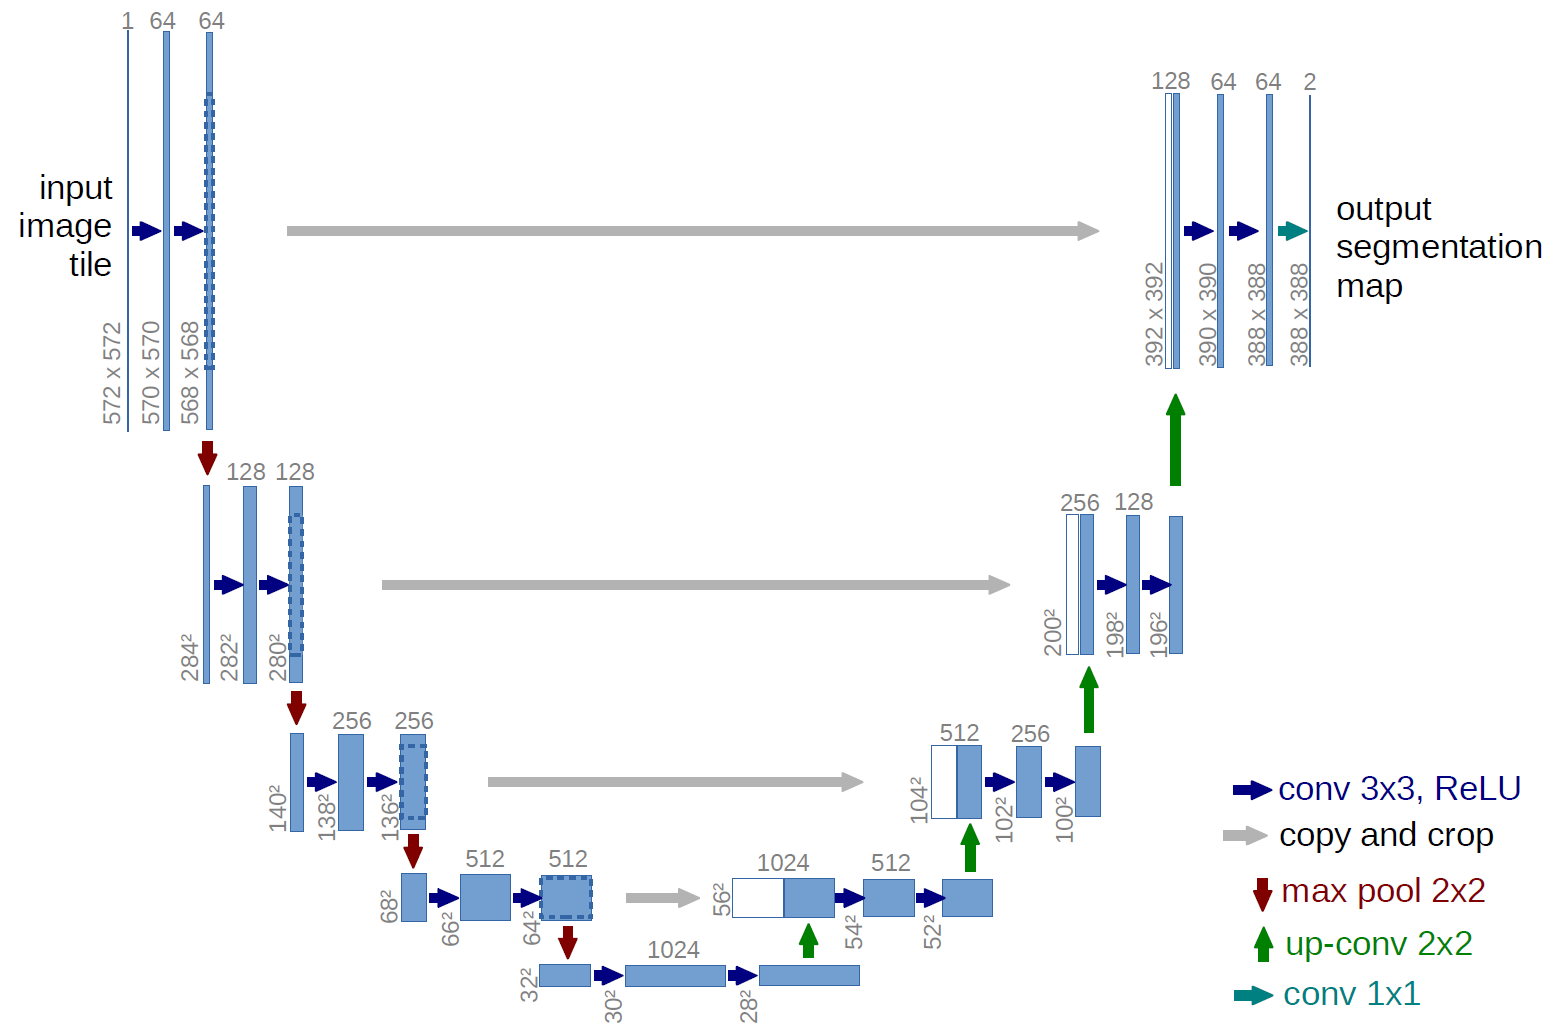
\includegraphics[scale=0.2]{u-net}
  \caption{Shows the U-Net architecture proposed by Ronneberger \textit{et al.} \parencite{ronneberger_u-net:_2015}.}\label{fig:unet}
\end{figure}
Notice that the size of the input image and the output prediction in \ref{fig:unet} is different. This is because the U-Net uses unpadded convolutions so at every convolutional layer one pixel is lost at every side. To obtain predictions in the borders of an image the context is extrapolated by mirroring the image \parencite{li_deepunet:_2017}. It is also important that we choose an initial image size so the activation maps length is even through all layers of the network. \parencite{ronneberger_u-net:_2015}. In theory the U-Net can handle images of any size but in practice we have memory limitations for the GPU. Large input images is therefore split up into patches. The segmentation on the patches can then be directly stitched together without any overlapping because the net uses unpadded convolutions.
\section{Classification networks}
For the discriminative part of the GAN a classification network is needed. This takes a input image and a set of segmentation maps and decides if the segmentation maps are artificial or ground truth. There are several high preforming classification networks such as the VGG networks \parencite{simonyan_very_2014} and the ResNet networks \parencite{he_deep_2015}.
\subsection{VGG Networks}
The popular 16 layer VGG16 or the 19 layers VGG19 have performed very well on a wide variety of tasks such as classification \parencite{simonyan_very_2014}. They have been used inside Fast Region-based Convolutional Networks (fast R-CNN) \parencite{ren_faster_2015, girshick_fast_2015} to generate object activation maps for the regional proposal network (RPN). Fast R-CNN have been able to do object detection and bounding box prediction at a fraction of the time of earlier networks. They have also been used as a encoder in the SegNet architecture which has been a very popular segmentation network \parencite{badrinarayanan_segnet:_2015}.
\begin{figure}[h!]
  \centering
      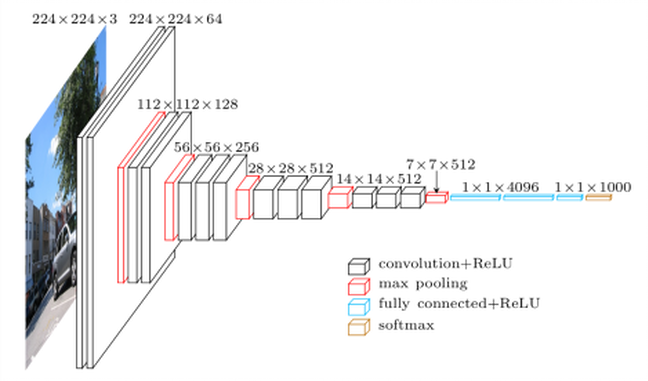
\includegraphics[scale=0.5]{vgg}
  \caption{The VGG16 architecture proposed by \cite{simonyan_very_2014}} \label{fig:vgg}
\end{figure}
The VGG16 network takes inputs of images with size $224 \times 224$ and produces a class wise prediction. The network is very simple, yet powerful and uses only $3 \times 3$ convolutions and $2 \times 2$ max pooling layers with stride 2.
\subsection{ResNet networks}
ResNet is another widely popular classification network. It has performed very well on classification tasks \parencite{he_identity_2016, szegedy_inception-v4_2016} It has also been shown that wider residual networks are more memory efficient while still obtaining comparable performance \parencite{wu_wider_2016, zagoruyko_wide_2016}.
\begin{figure}[h!]
  \centering
      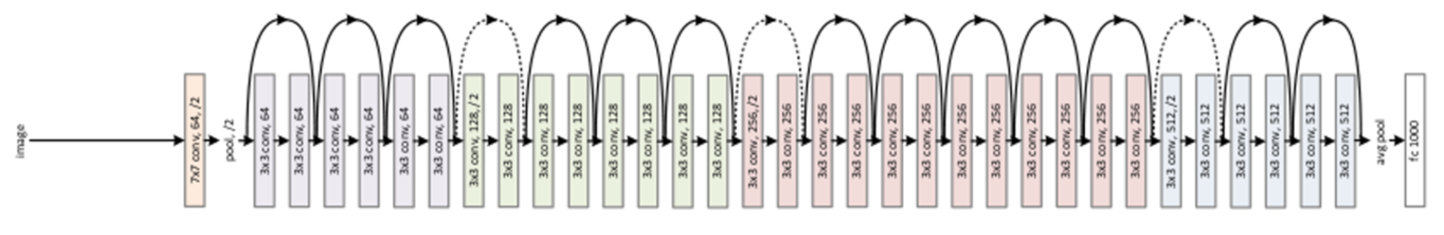
\includegraphics[scale=0.25]{resnet}
  \caption{The 34 layer deep ResNet architecture \parencite{simonyan_very_2014}} \label{fig:vgg}
\end{figure}
The success behind the ResNet lies in the residual blocks. A residual block is a two or more convolutional layers with a identity short-cut connection in between. The residual block can be defined as.
\begin{equation}
y=F(x, W) + x
\end{equation}
The benefit of this is that this guarantees that the gradients will flow through the entire network. Therefore, it is possible to build and train very deep residual networks by stacking hundreds of residual blocks. This also allows the network to itself decide the required depth since it can learn to set the weight of the final residual blocks to zero if they are not needed \parencite{he_deep_2015}. Hence, we get a very flexible network where we easily can adapt the depth to the task at hand.
\section{Weight functions and dealing with severely imbalanced datasets}
Due to the nature of overhead images the objects of interest are usually small compared to the entire image. This causes the dataset to be imbalanced since most pixels will belong to the background class. A naive segmentation network could then obtain good accuracy by only predicting everything to the background class. To combat this there are several techniques. The most straight forward is to use a weighted cross entropy loss where every term is weighted depending on the class frequency \parencite{sudre_generalised_2017}. Below is the weighted cross entropy loss for a two class segmentation problem.
\begin{equation}
\ell_{wce}(\hat{y}, y)=-\omega_cylog(\hat{y}) + (1-y)log(1-\hat{y})
\end{equation}
Here $y$ is the true probability for the foreground class, $\hat{y}$ the predicted probability for the foreground class and $\omega_c$ the class weights for the foreground class depending on the frequency which can be defined in many different ways such as. 
\begin{equation}\label{eq:wc1}
w_c=\frac{W*H - \sum_{x=0}^{W*H} \hat{y}_{c=1}(x)}{\sum_{x=0}^{W*H} \hat{y}_{c=1}(x)}
\end{equation}
Here W and H are the width and height of the image and $\hat{y}_{c=1}(x)$ the predicted probability that pixel x belongs to class one.
\begin{equation}\label{eq:wc2}
w_c=\frac{\sum_{n=0}^{N} \sum_{x=0}^{W*H} y_{c=0}(x)}{\sum_{n=0}^{N} \sum_{x=0}^{W*H} y_{c=1}(x)}
\end{equation}
Which is the sum over all of the background pixels in the training dataset divided by the foreground pixels.
Another popular approach is to minimize the intersect over union loss \parencite{yu_unitbox:_2016, rahman_optimizing_2016}. The intersect over union loss for a two class segmentation task is given below.
\begin{equation}
\ell_{IoU}(\hat{y}, y)= 1 - \frac{ \sum_{x=0}^{W*H} y(x)*\hat{y}(x) }{ \sum_{x=0}^{W*H} y(x) + \sum_{x=0}^{W*H} \hat{y}(x) - \sum_{W*H} y(x) * \hat{y}(x)}
\end{equation}
Here $\hat{y}(x)$ is the discrete class prediction for pixel x.\\
\\
To ensure good object separation Ronneberger \textit{et al.} \parencite{ronneberger_u-net:_2015} proposes to scale the pixel wise loss based on the proximity to the closet two foreground objects according to.
\begin{equation}\label{eq:pxl_weight}
	\ell_{pxl}(\hat{y}, y) = - \sum_{x=0}^{H*W}\omega(x)*y(x)*log(\hat{y}(x))
\end{equation}
Here $\omega(x)$ is the weighting term for pixel x, $y$ is the one hot encoding for the class of pixel x, $\hat{y}(x)$ is the prediction for pixel x and $H$ and $W$ is the height and width of the segmentation map. The weighting factor $\omega(x)$ is computed as following.
\begin{equation}\label{eq:weight}
\omega(x)=\omega_c+\omega_0*epx(\frac{(-d_1(x)-d_2(x))^{2}}{2\sigma^2})
\end{equation}
Here $\omega_c(x)$ depends on the class frequency and could be computed as \ref{eq:wc1} or \ref{eq:wc2}. The distances $d_1(x)$ and $d_2(x)$ is the distance to the nearest and second nearest foreground object. The constant $\sigma$ determines how fast the penalty should decay with increasing distance and $\omega_0$ is a coefficient that determines the importance of the object separation penalty.

\section{Earlier work}
In most cases the segmentation networks needs some post processing to improve the accuracy of the segmentation maps. Conditional random markov fields CRF have been very successfully to enforce spatial contiguity in the output maps \parencite{arnab_higher_2015, luc_semantic_2016}. There have been work that used mean field inference expressed as a recurrent convolutional networks to do CRF like post processing \parencite{schwing_fully_2015, zheng_conditional_2015}. Luc \textit{et al.} \parencite{luc_semantic_2016} proposed a adversarial segmentation network to enforce higher order potentials without being limited to a single class. Instead, of directly enforcing these higher order potentials in a CRF model as post processing the goal was to enforce them in the generator directly with adversarial training. This technique also has the benefit of lower complexity since at test time only the generator will be used.\\
\\
The generators task was to produce segmentation maps for the C classes. One initial concern was that the discriminator would trivially be able to differentiate the generated segmentation maps from the ground truth by only examining if they were continuous or discrete. To combat this a scaling method was proposed where the ground truth segmentation maps were processed so that a mass of $\tau$ where placed on the correct label but were otherwise made as similar as possible to the generated maps (in regard to KL divergence). The scaling method showed no improvement over the basic method with no preprocessing.\\
\\
Son and Jung \textit{et al.} \parencite{son_retinal_2017} showed that a U-NET combined with an adversarial loss could achieve state of the art performance for retinal vessel segmentation in fundoscopic images. The team investigated several types on adversarial networks proposed in \parencite{isola_image--image_2016} such as image-GAN, patch-GAN and pixel-GAN. For Image-GAN the discriminator make a decision on a image level if the image is generated or not. For patch-GAN the images are split into patches and the discriminator analyses each individually. The result is the aggregated result from all patches. For pixel-GAN the discriminator makes it decision on pixel per pixel level. The team found that a image-GAN together with a cross entropy term preformed the best and outperformed the non adversarial segmentation network trained only with the cross entropy loss by a small margin.\\
\\
Ronneberger \textit{et al.} \parencite{ronneberger_u-net:_2015} showed that a U-NET could learn small border pixels in cell segmentation by weighting the loss as \ref{eq:pxl_weight}. The loss enforced the network to learn small border and outperformed the second best network on the ISBI cell tracking challenge 2015 with a large margin.
\chapter{Method}
\section{The segmentation network}
\subsection{Network architecture}
For the segmentation network a U-Net proposed by \parencite{ronneberger_u-net:_2015} was used. Different number of filters in the initial layer was tried but it was concluded that more than 16 filters did not give a better performance but instead only resulted in a greater computational cost and greater over fitting. Dropout did not manage to solve the over fitting problem for the more complex networks so a U-Net with 16 initial filters and no dropout was chosen as the segmentation network for the following experiments. To produce data augmentation the training image were randomly rotated 0, 90 180 or 270 degrees as well as randomly mirrored left to right and up to down.\\
\\
To extract vehicles from the segmentation map connected component extraction is used. Pixels can be defined to be connected by four or eight way connectivity. In four way connectivity only the above, below and two sideways neighbours are examined for connectivity but in eight way connectivity the diagonal neighbours are examined as well. Since all pixels in a vehicle should be four way connected with each other we will only use this mode. The most simple and intuitive method of extracting connected components in an image is the two pass algorithm \parencite{stockman_computer_2001} which is a O(n) time algorithm. The below image shows the proposed pipeline at testing time for counting and detecting vehicles.
\begin{figure}[H]
  \centering
      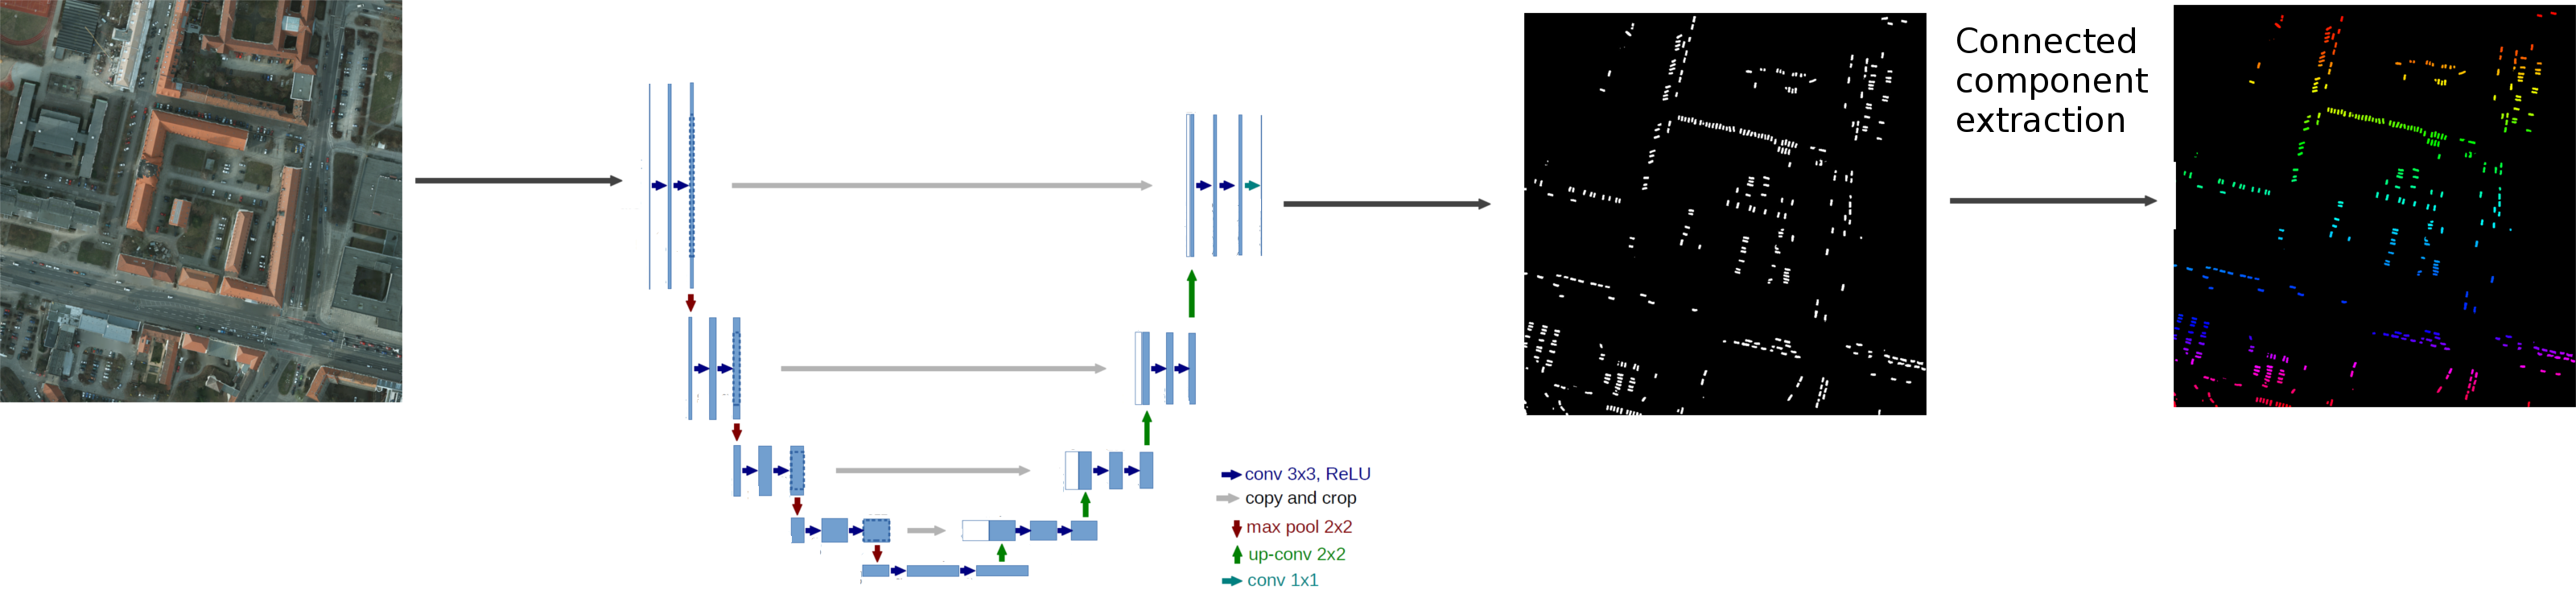
\includegraphics[scale=.16]{net}
  \caption{The 34 layer deep ResNet architecture \parencite{simonyan_very_2014}} \label{fig:vgg}
\end{figure}
\subsection{Border mirroring}
Since the U-Net uses unpadded convolutions the output segmentation is smaller than the input image. Therefore, borders were added to the input image to give the output segmentation the desired size. Information in the borders where extrapolated by mirroring. The below image shows the result of mirroring borders. The mirrored borders are shaded for clarity and the lighter are is the covered area for the output segmentation map.
\begin{figure}[H]
  \centering
      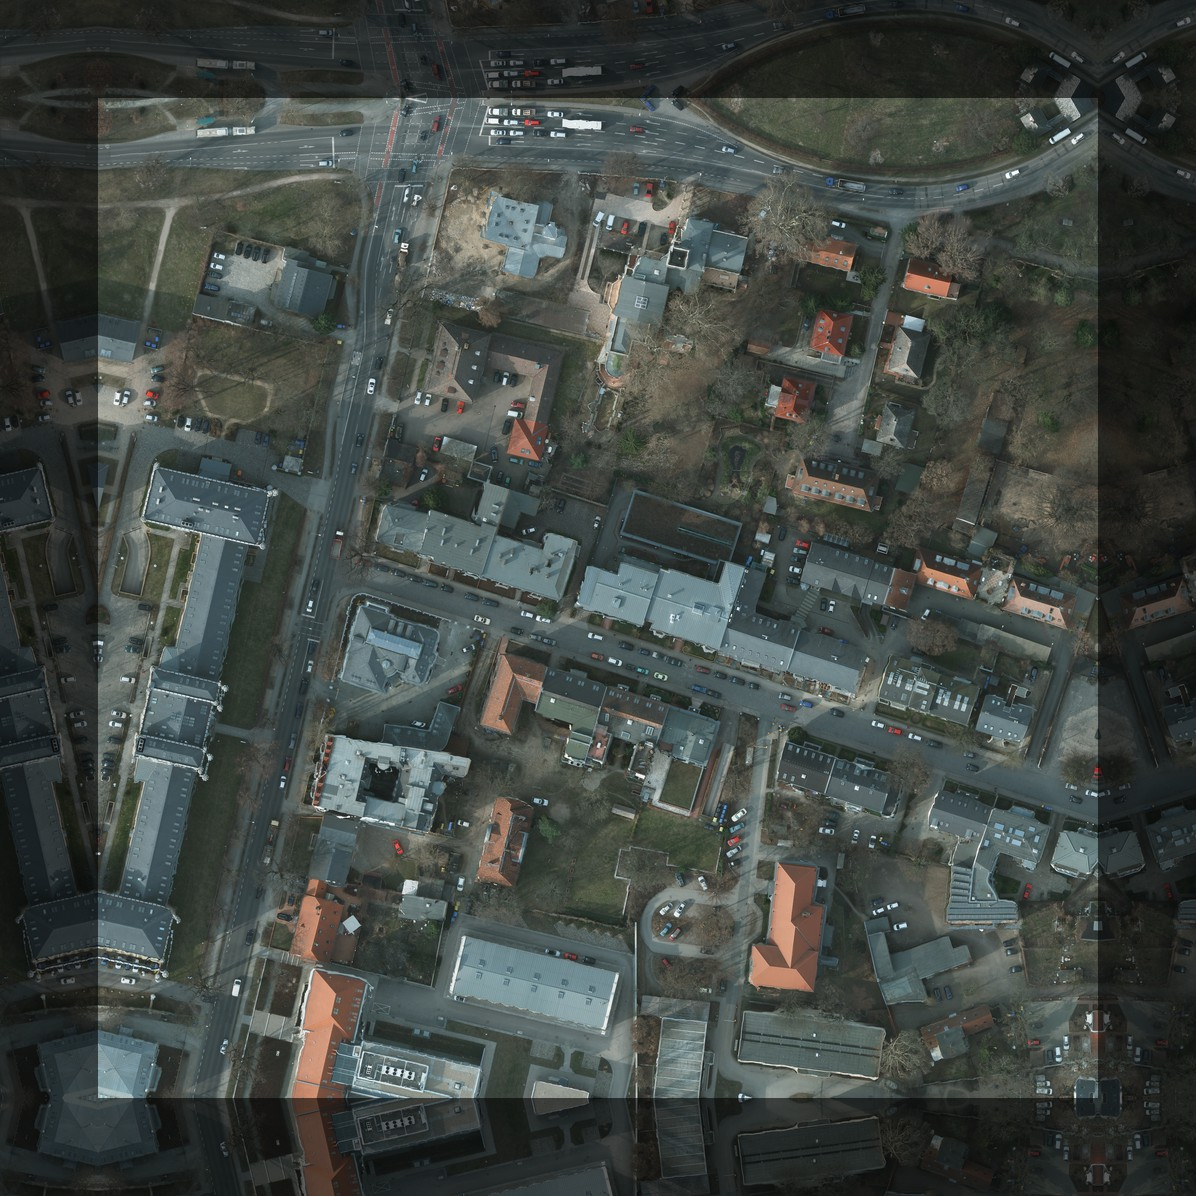
\includegraphics[scale=.8]{borders}
  \caption{Shows a training image with mirrored borders from the Potsdam dataset. The shaded area will be lost due to unpaded convolutions} \label{fig:vgg}
\end{figure}

\section{Weighting the cross entropy loss}
Using the weighting definition \ref{eq:pxl_weight} the cross entropy loss was weighted based on object separation. Initially $\omega_c$ was set to reflect the class imbalance as defined in \eqref{eq:wc1} or \eqref{eq:wc2}. This led the model to achieve a good recall but a low precision and F1 score. The values $\omega_c =2$, $\omega_0=10$ and $\sigma=3$ was found to give a good F1 score while also enforcing better object separation. Below is the binary labels a well as the corresponding weight map for each pixel for the given values.
\begin{figure}[H]
\minipage{0.45\textwidth}
  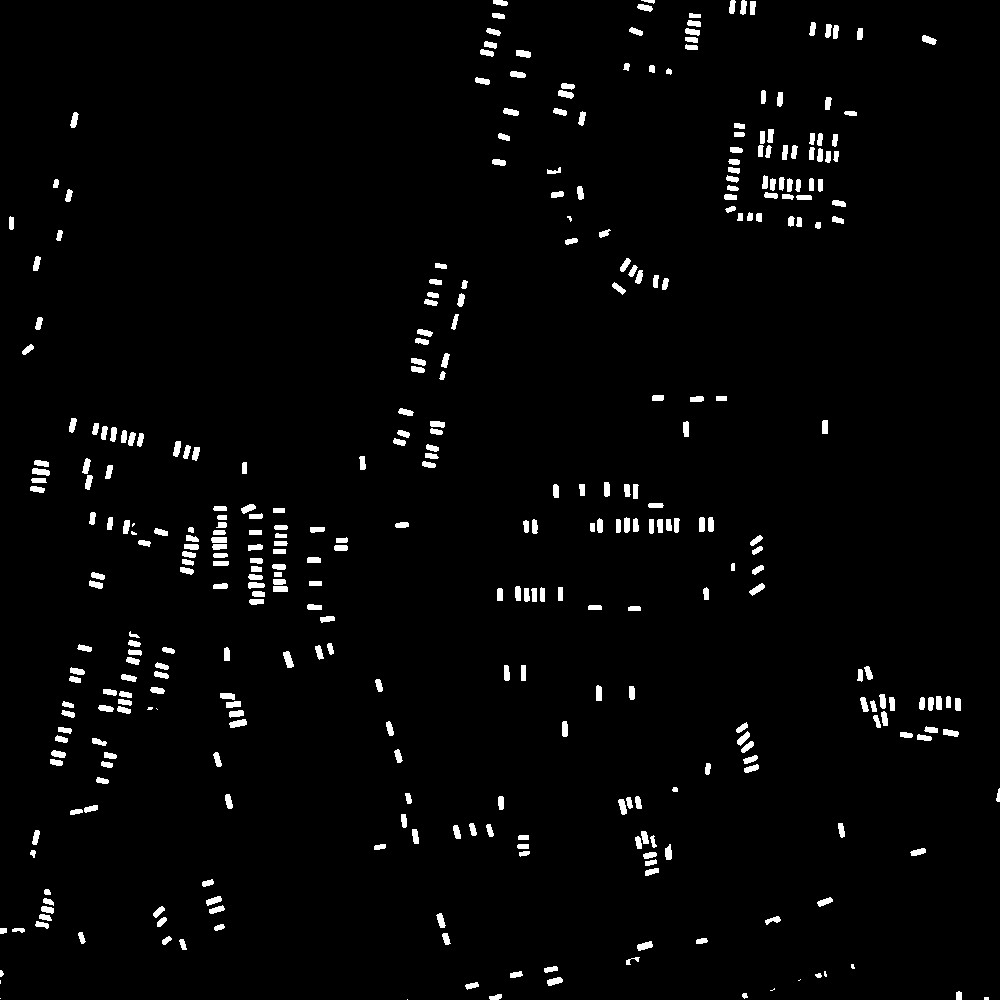
\includegraphics[width=\linewidth]{weight_labels}
%  Image \textbf{(a)}, the input validation image
\endminipage\hfill
\minipage{0.53\textwidth}
  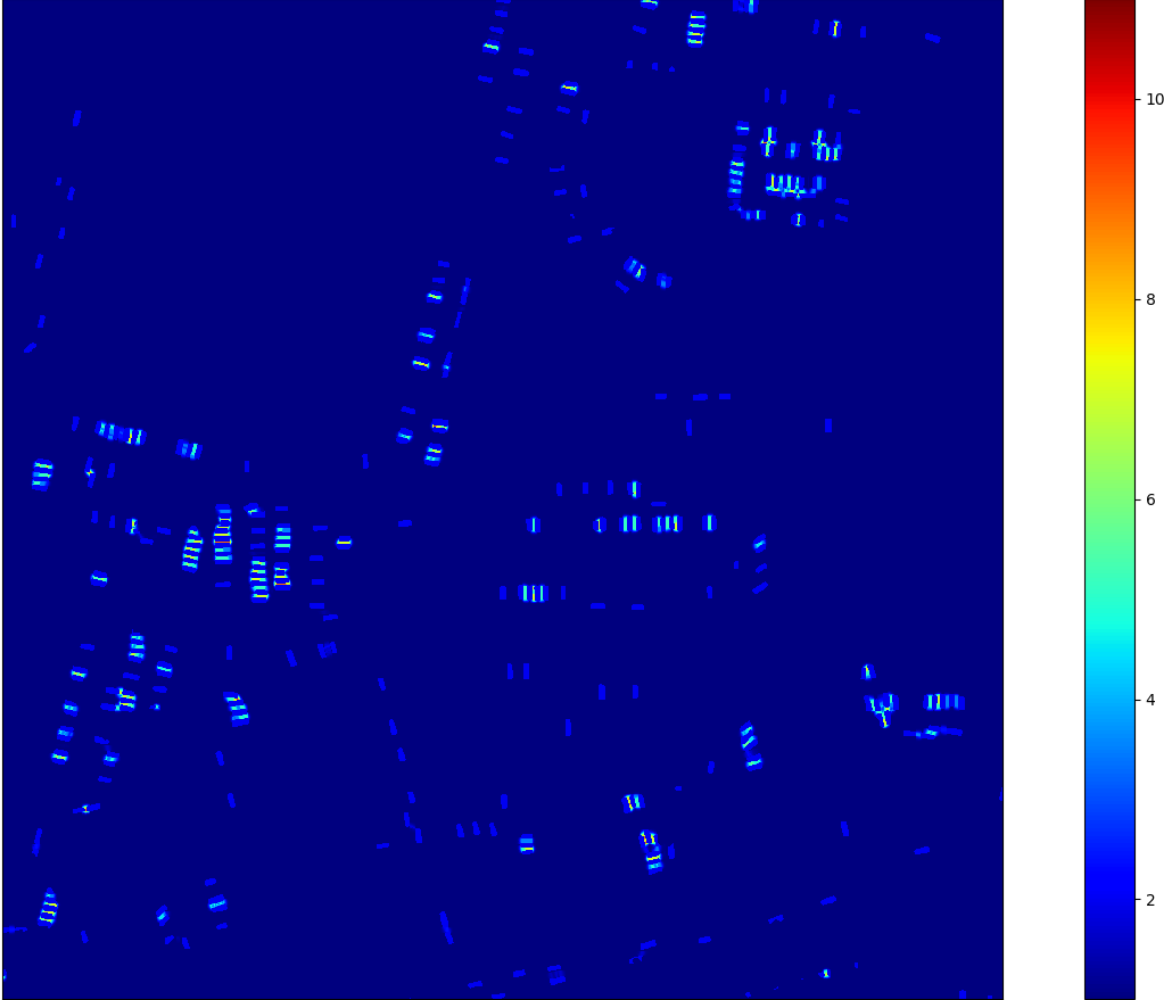
\includegraphics[width=\linewidth]{weight_map_3}
%  Image \textbf{(b)}, the ground truth segmentation
\endminipage\hfill
\caption{Figure shows the ground truth labels and the pixel weight map for a training image.}
\end{figure}
\section{Adding an adversarial loss term}
For the discriminative network a ResNet will be used. The ResNet is chosen over the VGG due to its slightly better performance and computational cost \parencite{johnson_cnn-benchmarks:_2018} as well as its flexible architecture which makes it easy to change the depth or the input size. The input to the discriminative network will be the satellite image concatenated with the ground truth or generated segmentation as showed in the image below. 
\begin{figure}[H]
  \centering
      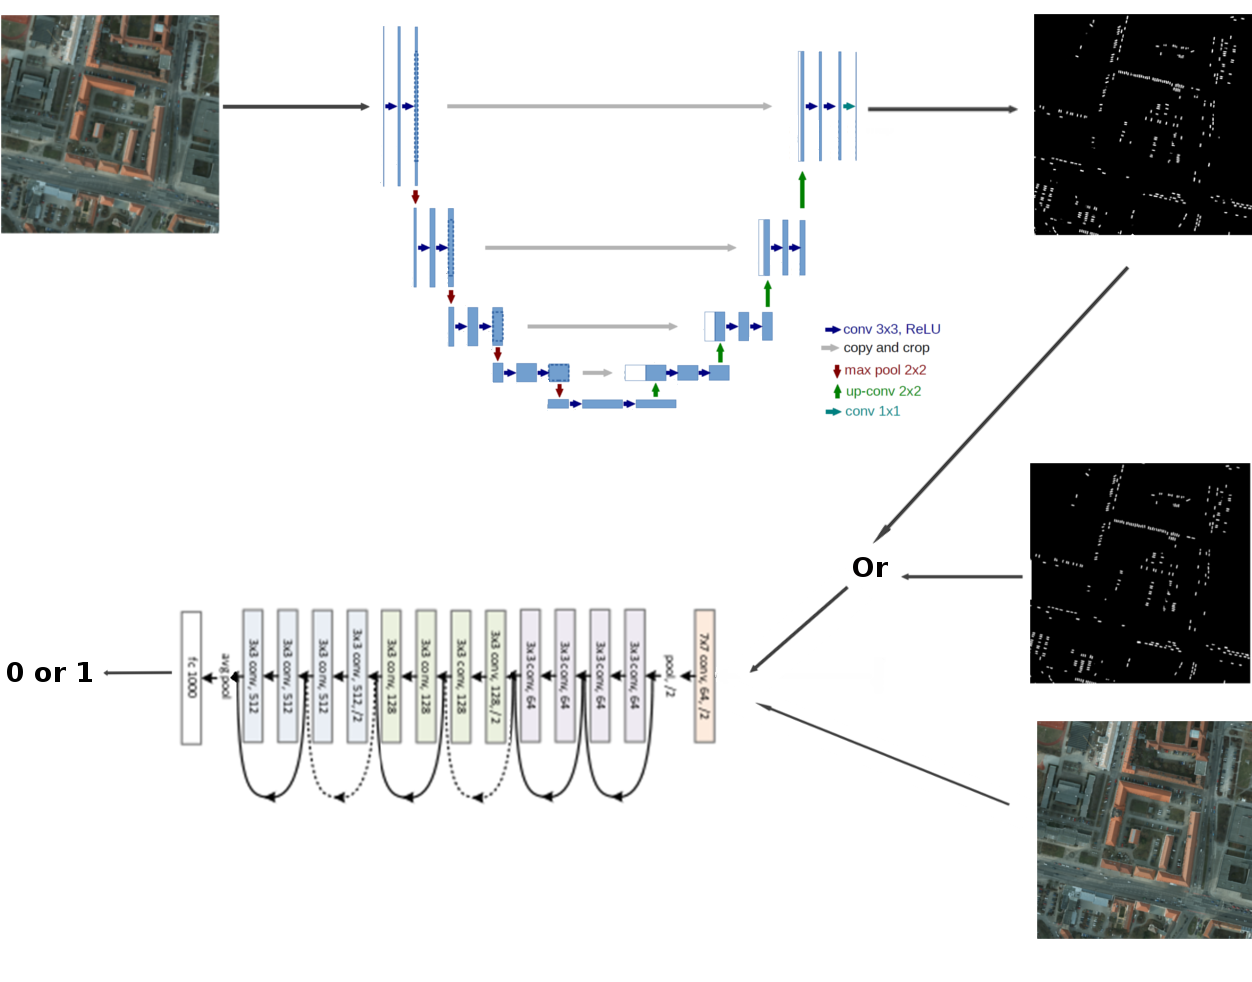
\includegraphics[scale=0.25]{gan_no_n}
  \caption{The 34 layer deep ResNet architecture \parencite{simonyan_very_2014}} \label{fig:vgg}
\end{figure}
A patch-Gan structure will be used where the discriminator will only have a view of $100 \times 100$ pixels at once. The loss for the discriminator will be the average loss over all patches. The reason for this is that a patch-Gan with a smaller window was more stable during training compared to a patch-Gan with a larger window or an image-Gan. This also made it easy to perform batch normalization over the batch of patches extracted from one image.\\
\\
Following the example of \cite{goodfellow_generative_2014, luc_semantic_2016} the term $-\ell_{bce}(D(G(x),y), 0)$  is replaced with  $+\ell_{bce}(D(G(x),y), 1)$ in equation \ref{eq:cgan}. Hence instead of minimizing the probability of the discriminative network to predict the generated map to be synthetic we maximize the probability of predicting the generated map as ground truth. The reason for this is that it leads a stronger gradient for the discriminator when making predictions on ground truth and generated maps. The objective function for the GAN becomes.
\begin{equation}
\Lagr_{bce}(G, D) =\lambda(\ell_{bce}(D(x,G(x)), 1)-\ell_{bce}(D(x,y), 1))
\end{equation}
Finally we define our minimax game as.
The objective for the network hence becomes.
\begin{equation}
G^{*}=argmin_{G}[\ell_{pxl}(G(x),y) + max_{D}[\lambda\Lagr(G, D)] ]
\end{equation}
\\
Here we set $\lambda=0.01$ since this value gave a low importance to the adversarial loss early in the training but a larger importance at later stages when the cross entropy loss had decreased significantly. This led to faster convergence of the network while training. The model converged a lot slower with a larger value on $\lambda$ since the adversarial network would place too much importance on one specific difference early in training and completely disregard other differences. For example, the discriminator might learn the average size of a vehicle and solely base its decision on this. The generator would then be able to decrease its loss significantly by only chopping up objects into vehicle sized object and disregarding the nature of the object.\\
\\
Since \cite{luc_semantic_2016} showed that there were no significant disadvantage of concatenating the generated maps with the satellite image in the basic manner opposed to the product or scaling method this was the initial approach. However in our experiments the discriminative network quickly learned to spot the difference between the discrete ground truth labels and the continuous generated labels and spent all of it's time teaching the generative network to draw discrete boundaries and almost completely disregarded the initial segmentation task. To force the discriminative network to learn a more productive loss function the ground truth labels were first smoothed before being fed into the discriminator. The smoothing were performed so that the ground truth labels should have the same smoothness in border pixels as the generated segmentation maps without an adversarial loss. This forced the discriminative network to learn a more productive loss function and greatly improved performance.\\
\\
Initially both models were updated at each step. However it turned out that the network complexities poorly matched each other and one network always ended up outperforming the other. Initially a U-NET with 64 kernels in the first layer was used. For the adversarial networks a ResNet with depth 14 18,34, 50 and 101 was tried but for all the configurations one of the networks drastically outperformed the other and training diverged as a result. To more easily be able to monitor the learning of the two networks the loss functions where changed to.
\begin{equation}
\Lagr(G) = \ell_{pxl}(G(x),y)+\lambda\ell_{bce}(D(x,G(x)), 1)
\end{equation}
\begin{equation}
\Lagr(D) =\ell_{bce}(D(x,G(x)), 0) + \ell_{bce}(D(x,y), 1)
\end{equation}
Here both networks tries to minimize its respective loss function. An alternating training regime described below could now be used.
\lstinputlisting[language=Python]{training.py}
Here \% is the modulus operator and $check\_discriminator=20$ and $cutoff=1.0$. Since we stop training the discriminative network when its loss goes below the cutoff value the discriminative network is not able to significantly outperform the generative network. A cutoff value of 1.0 indicates that the discriminative network makes a correct prediction approximately 60\% of the time.\\

\chapter{Result}
\section{The datasets}
\subsection{The ISPRS Potsdam semantic dataset}
The ISPRS Potsdam dataset is a two dimensional semantic segmentation
dataset \cite{noauthor_2d_nodate}. The dataset has six classes, impervious surfaces, buildings, low, vegetation, trees, cars and clutter/background. The images are are of the TIFF format and has $6000 \times 6000$ resolution with a resoloution of 5 cm per pixel. There are 24 images for training
and validation and 14 for testing. The images are rgb or infra-red together
with rgb. There is also a height data channel. The ground truth segmentation for the test images is not released and the segmentation maps have to be sent to ISPRS for evaluation. Below is an example of the training data from the ISPRS Potsdam semantic dataset.
\begin{center}
\begin{figure}[H]
      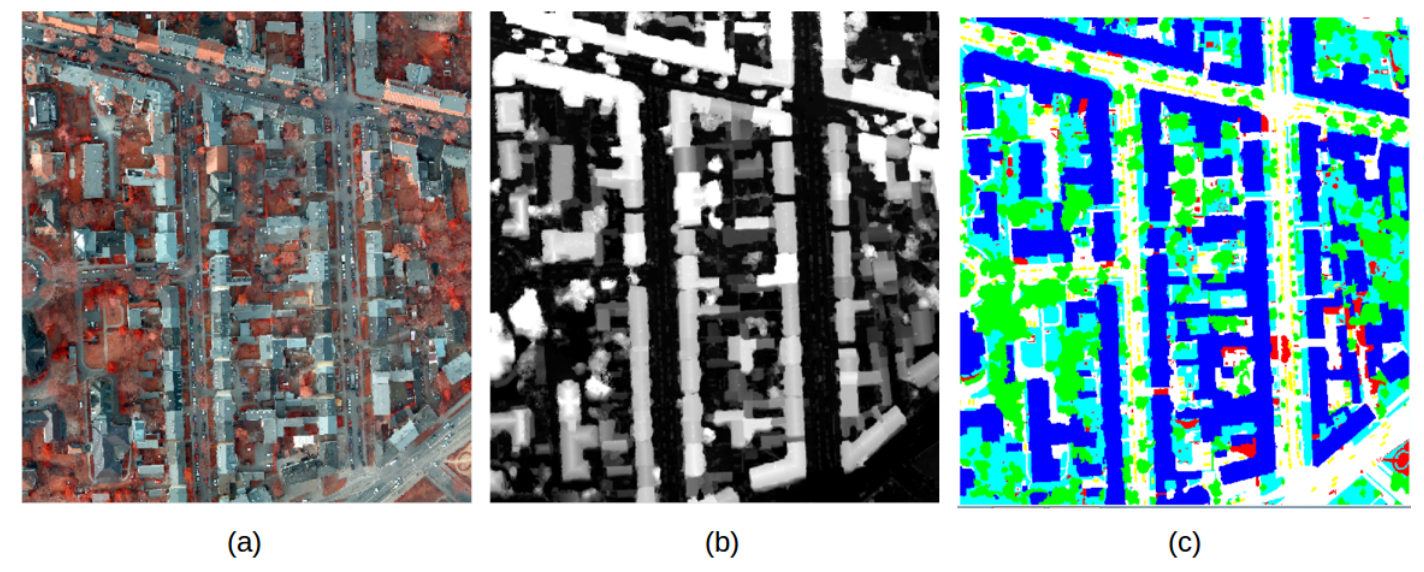
\includegraphics[scale=0.25]{potsdam}
  \caption{An example image from the Potsdam dataset with a: the rgb
channel, b: the height data channel and c: the ground truth segmentation
map.}
\end{figure}
\end{center}
The evaluation metric for the individual classes is pixel wise F1 score and the
overall performance is measured by pixel accuracy.
\begin{equation}\label{eq:precision}
Precision=\frac{True\textit{ }positive}{True\textit{ }Positive+False\textit{ }poitive}
\end{equation}
\begin{equation}\label{eq:recall}
Recall=\frac{True\textit{ }positive}{True\textit{ }Positive+False\textit{ }negative}
\end{equation}
\begin{equation}\label{eq:f1}
F1\textit{ }score=\frac{2*Recall*Precision}{Recall+Precision}
\end{equation}
This work focuses on detecting vehicles in low cost images so the images will be down sampled to a resolution of $1000 \times 1000$ pixels which corresponds a resolution of 30 cm per pixel. This is done to match the resolution to the the resolution of commercial satellites such as DigitalGlobes WorldView 3 and 4 \cite{noauthor_worldview-3_nodate}. Only the car class will also be predicted. One important factor to keep in mind is that this is a multi class semantic dataset and not a vehicles detection dataset. In several of the images it is possible to spot vehicles through trees without leaves but these are not segmented as vehicles but as trees. This makes it a harder challenge for the semantic network since it must learn to differentiate between very similar objects.
\begin{figure}[H]
\minipage{0.48\textwidth}
  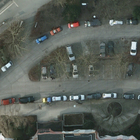
\includegraphics[width=\linewidth]{trees}
  Image \textbf{(a)}, the input validation image
\endminipage\hfill
\minipage{0.48\textwidth}
  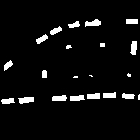
\includegraphics[width=\linewidth]{trees_label}
  Image \textbf{(b)}, the ground truth segmentation
\endminipage\hfill
\caption{Figure shows the ground truth labels and the pixel weight map for a training image}
\end{figure}
\subsection{The VEDAI dataset}
The VEDAI dataset \cite{razakarivony_vehicle_2015} consists of 9 different classes, these classes and the number of objects are given in the table below.\begin{center}
\begin{tabular}{|c|c|}
\hline
\textbf{Classes} & \textbf{Number}\\
\hline
Car & 1340\\
Pick-up & 950\\
Truck & 300\\
Plane & 47\\
Boat & 170\\
Camping car & 390\\
Tractor & 190\\
Vans & 100\\
Other & 100\\
\hline
\end{tabular}
\end{center}
To make the results comparable with the extensive research of different methods done by \cite{zhong_robust_2017} the classes plane, boat tractor van and other were removed due to scarcity of data.  The annotations for each target consists on the centre coordinates of the target the angle of the center line of the bounding box as well as the corners of the bounding box. The bounding box fits the target closely so no extra information is given on the sides. The evaluation metrics on the VEDAI dataset are precision recall and F1-score:\\
\\
The dataset was divided into three parts where 927 images were used for training, 100 for validation and 240 for testing. The dataset was transformed into a semantic dataset by assigning the pixels of the bounding boxes for remaining classes to the foreground class and the rest of the pixels to the background class. A small ''artificial'' separation was introduced around each bounding box so that all bounding boxes would be separated in the ground truth segmentation.\\
\\
The dataset is severely imbalanced and around 99.3 \% of all pixels belongs to the background class. To deal with this the training data set was first filtered to make it more balanced. From the 927 training images only those which contained five or more vehicles where selected which resulted in 166 images. Those images where used for the initial part of training and when the network started overfitting and the performance on the validation data decreased the network was finally trained on all of the training images. This training procedure removed instabilities early on in training where the network otherwise where inclined to predict everything to the background class and set all weights to zero.
\section{Weighting the loss function}
The network with the weighted cross entropy loss achieved a comparable f1 score with the original network but but learned to separate objects much better. In the below segmentations we use discrete predictions to better display object separations.
\begin{center}
\begin{figure}[H]
      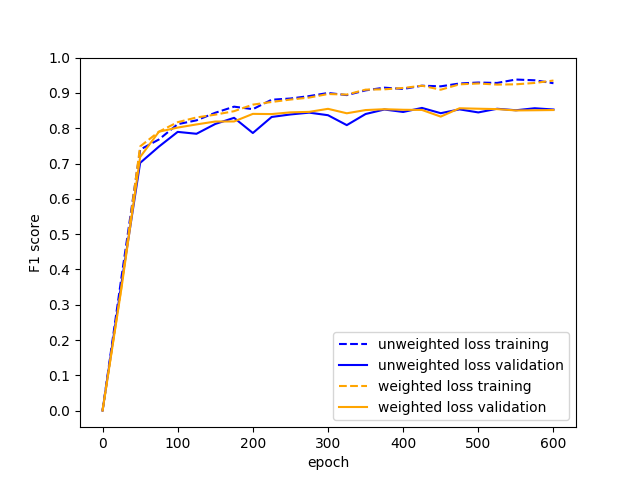
\includegraphics[scale=0.7]{weighted_vs_unweighted}
  \caption{} \label{fig:weighted_vs_unweighted}
\end{figure}
\end{center}
\begin{figure}[H]
\minipage{0.32\textwidth}
  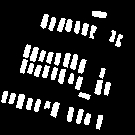
\includegraphics[width=\linewidth]{class_vs_w/label_1}
\endminipage\hfill
\minipage{0.32\textwidth}
  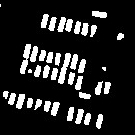
\includegraphics[width=\linewidth]{class_vs_w/un_weight_1}
\endminipage\hfill
\minipage{0.32\textwidth}%
  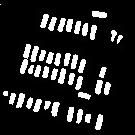
\includegraphics[width=\linewidth]{class_vs_w/weight_1}
\endminipage
\caption{}
\end{figure}

\begin{figure}[H]
\minipage{0.32\textwidth}
  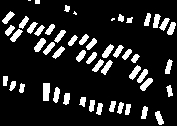
\includegraphics[width=\linewidth]{class_vs_w/label_2}
\endminipage\hfill
\minipage{0.32\textwidth}
  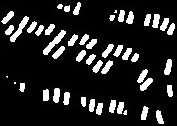
\includegraphics[width=\linewidth]{class_vs_w/un_weight_2}
\endminipage\hfill
\minipage{0.32\textwidth}%
  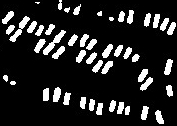
\includegraphics[width=\linewidth]{class_vs_w/weight_2}
\endminipage
\caption{}
\end{figure}
\begin{center}
\begin{tabular}{|c c c c c c c|}
\hline
\textbf{Tile \#} & 2\_11  & 2\_12 & 7\_9 & 7\_10 & 7\_11 & 7\_12 \\
\hline
\textbf{Number of vehicles} & 107 & 123 & 304 & 250 & 346 & 346 \\
\textbf{Predicted number of vehicles} & 108 & 126 & 310 & 251 & 352 & 337 \\
\textbf{Prediction error in \%} &0.9 &  2.4 & 1.9 & 0.4 & 1.7 & 2.7\\
\hline
\end{tabular}
\end{center}
\section{Adding an adversarial loss term}
Since the GAN game becomes unstable with sparse gradients the Relu activation function was therefore replaced with a leaky relu activation in both the generative and discriminative network and max pooling was replaced by mean pooling in the generative network. The U-NET already uses 2D transposed convolution for up sampling so this was kept as in the original network. This changes greatly stabilized the training. However I still managed to train a GAN using the origin U-NET with sparse gradients with a carefully chosen learning rate decay. This training was very unstable and even a small change in the learning rate would cause the training to diverge. Below is the F1 score on the validation data for both types of GANs.
\begin{center}
\begin{figure}[H]
      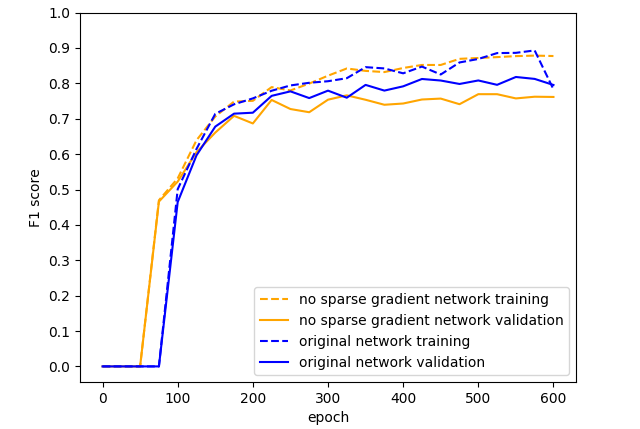
\includegraphics[scale=0.7]{mean_max_2}
  \caption{The VGG16 architecture proposed by \cite{simonyan_very_2014}} \label{fig:vgg}
\end{figure}
\end{center}
Both networks had a similar performance on the training data but the original network over fitted less and performed better on the validation data. Hence the original U-NET network was chosen as the generative network for the following comparisons although it was harder to train.
In the below plots we displays the segmentation as a continuous values where the brightness of each pixel is the probability that that pixel belongs to a car to make better comparisons between the two networks. To obtain a discrete prediction an argmax between this layer and the background class can be preformed. The segmented images looks very similar on a large scale.
\begin{figure}[H]
\minipage{0.48\textwidth}
  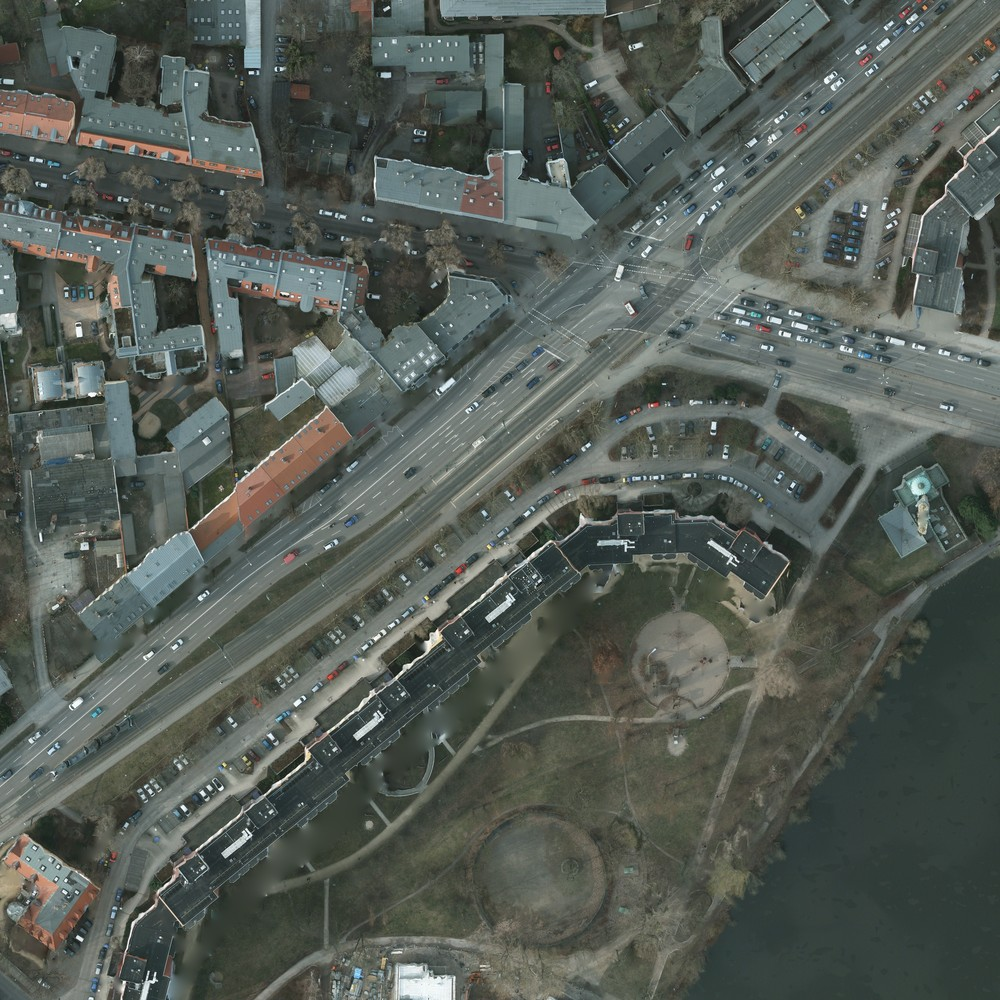
\includegraphics[width=\linewidth]{gan_vs_class/img_4}
  Image \textbf{(a)}, the input validation image
\endminipage\hfill
\minipage{0.48\textwidth}
  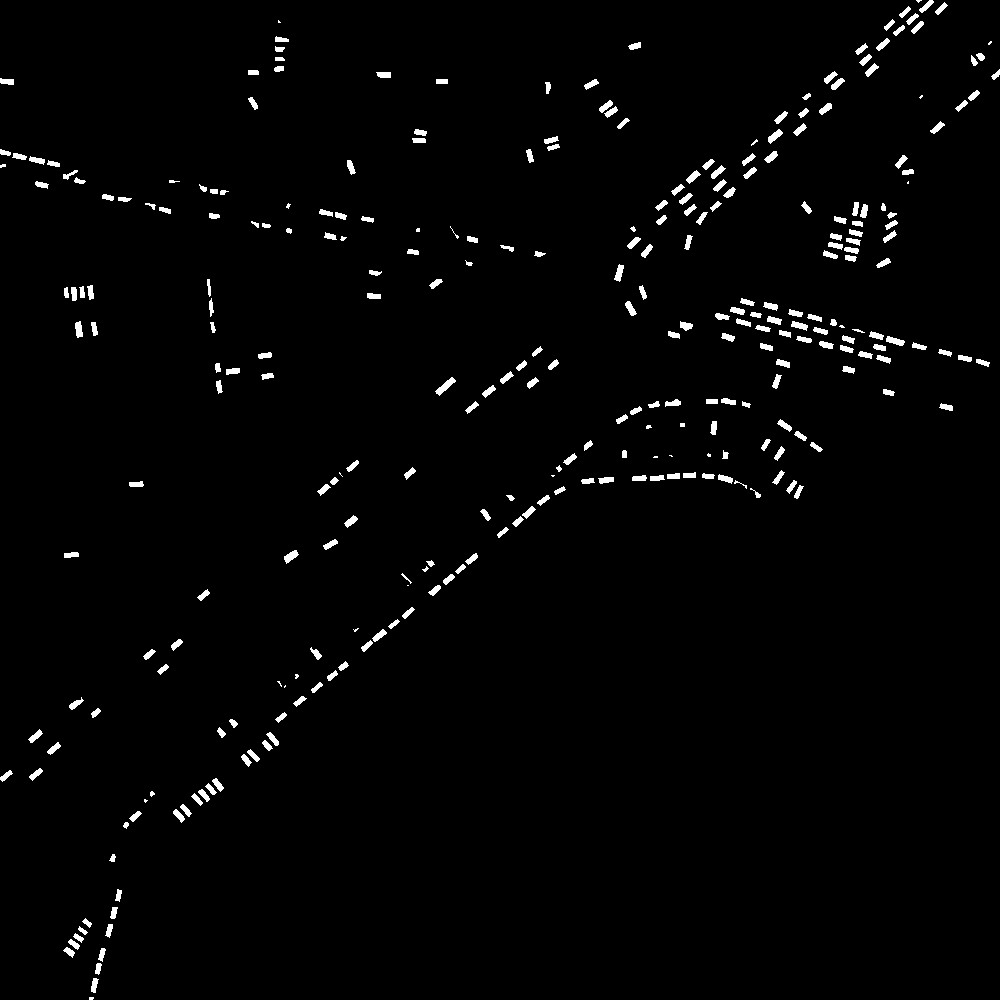
\includegraphics[width=\linewidth]{gan_vs_class/label_4}
  Image \textbf{(b)}, the ground truth segmentation
\endminipage\hfill
\minipage{0.48\textwidth}
  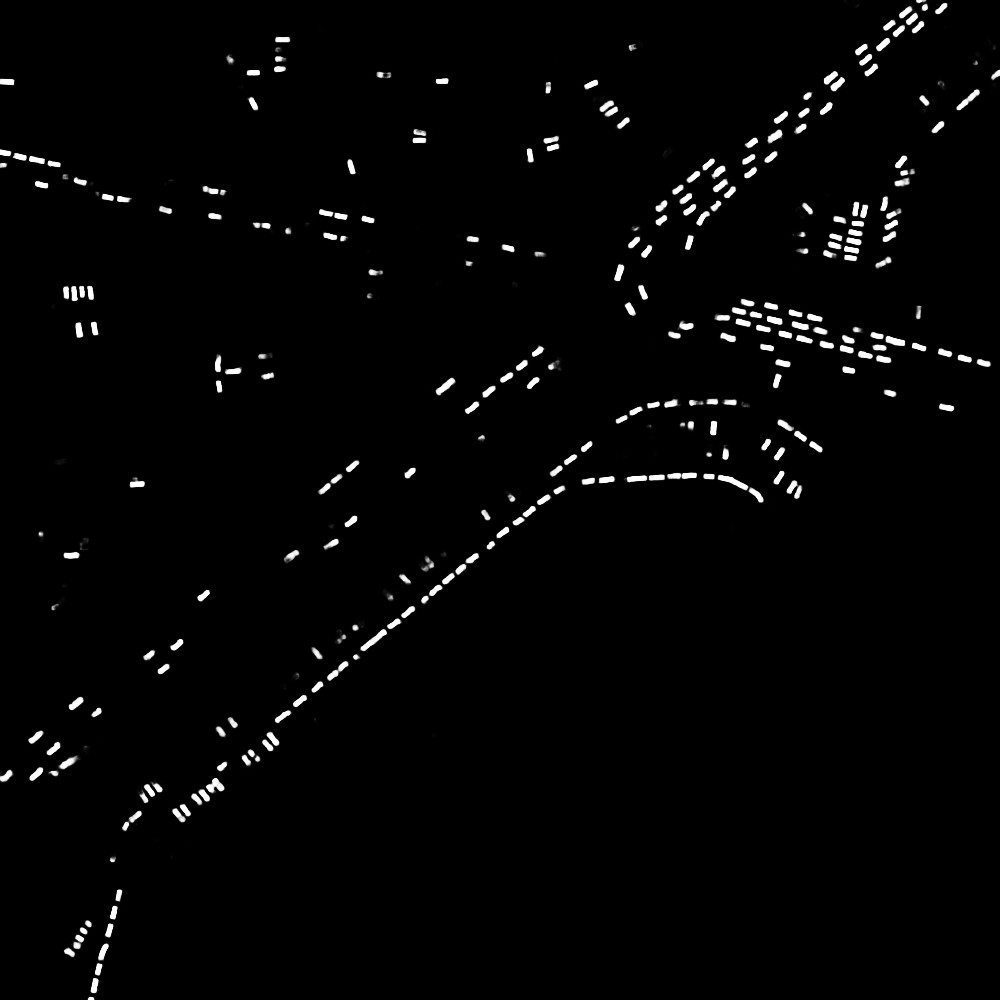
\includegraphics[width=\linewidth]{gan_vs_class/class_4}
  Image \textbf{(c)}, segmentation without an adversarial loss
\endminipage\hfill
\minipage{0.48\textwidth}%
  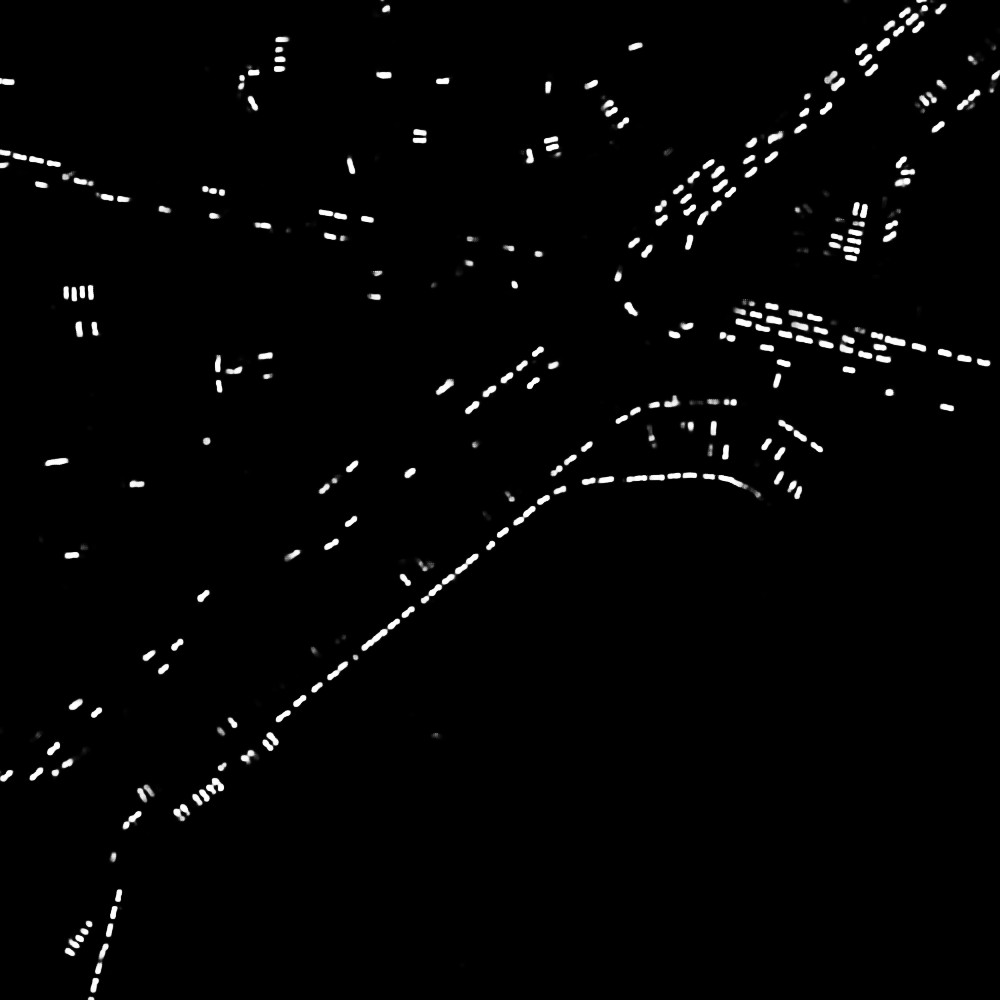
\includegraphics[width=\linewidth]{gan_vs_class/gan_4}
   Image \textbf{(d)}, segmentation with an adversarial loss
\endminipage
\caption{Figure \ref{fig:class_1} shows the ground truth segmentation,}
\end{figure}
However if we look closely there are differences between the two networks. The adversarial network managed to enforce more assertive predictions and cars were more likely to be fully segmented or completely left out. However the segmented objects seemed to be more loosely conditioned on the input image then for the network without an adversarial loss. Other differences were that the GAN network was more inclined to chop up false positives into vehicle like objects. It also had a tenancy to separate long vehicles such as trucks into smaller car like parts. Below are cherry picked images which displays the differences of the two networks. adversarial loss.
\begin{figure}[H]
\minipage{0.32\textwidth}
  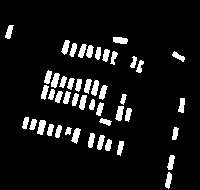
\includegraphics[width=\linewidth]{gan_vs_class/label_1}
\endminipage\hfill
\minipage{0.32\textwidth}
  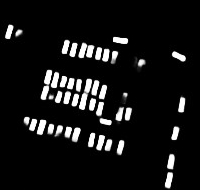
\includegraphics[width=\linewidth]{gan_vs_class/class_1}
\endminipage\hfill
\minipage{0.32\textwidth}%
  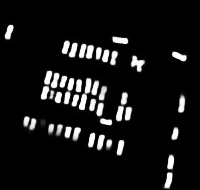
\includegraphics[width=\linewidth]{gan_vs_class/gan_1}
\endminipage
\caption{Figure \ref{fig:class_1} shows the ground truth segmentation, }
\end{figure}

\begin{figure}[H]
\minipage{0.32\textwidth}
  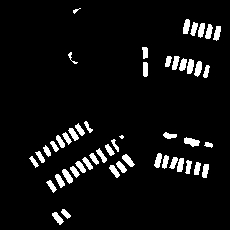
\includegraphics[width=\linewidth]{gan_vs_class/label_2}
\endminipage\hfill
\minipage{0.32\textwidth}
  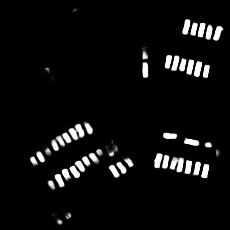
\includegraphics[width=\linewidth]{gan_vs_class/class_2}
\endminipage\hfill
\minipage{0.32\textwidth}%
  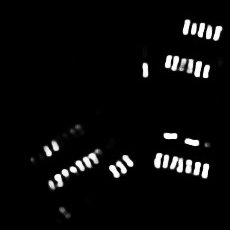
\includegraphics[width=\linewidth]{gan_vs_class/gan_2}
\endminipage
\caption{Figure \ref{fig:class_1} shows the ground truth segmentation, }
\end{figure}
When comparing the f1 scores the adversarial loss proved not to be helpful.
\begin{center}
\begin{figure}[H]
      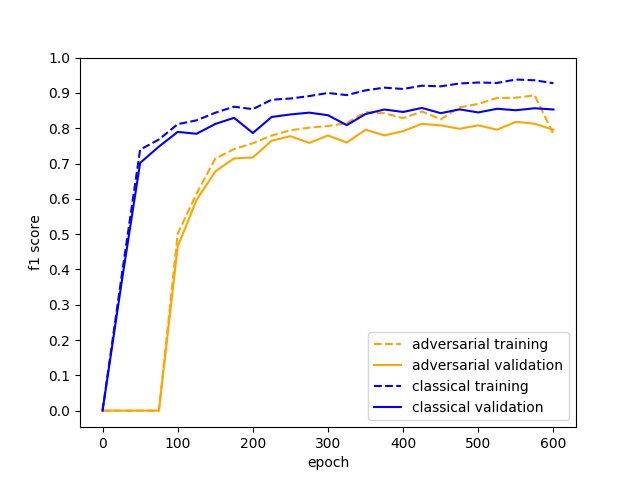
\includegraphics[scale=0.6]{classical_vs_adversarial}
  \caption{The VGG16 architecture proposed by \cite{simonyan_very_2014}} \label{fig:gan_vs_class}
\end{figure}
\end{center}
\section{Comparison with earlier work}
\newpage
\begin{center}
\captionof*{table}{Comparison on the ISPRS Potsdam dataset} \label{tab:potsdam} 
\begin{tabular}{|c | c | c|}
\hline
\textbf{Model} & Proposed Model & SBD \\
\textbf{Resolution used} & \textbf{30 cm/pixel} & 12.5 cm/pixel\\
\textbf{Pixel wise F1 score} & 0.851 & \textbf{0.884}\\
\textbf{Vehicle wise F1 score} & \textbf{0.811} &  0.773\\
\textbf{Mean prediction error counting cars} & \textbf{1.67 \%} &  3.57 \%\\
\textbf{Evaluation time per image *} & \textbf{0.19 seconds} &  28.19 seconds\\
\hline
\end{tabular}\caption{Shows the comparison between the proposed model and the Segment before you Detect (SBD) model \parencite{audebert_usability_2016} on the Potsdam dataset.\\ \textbf{*} The SBD model was evaluated on a Tesla K20 which can at maximum perform $3.52*10^{12}$ 32 bit floating point operations per second. The proposed model was evaluated on a Tesla K80 wich can perform at maximum $8.74*10^{12}$ 32 bit floating point operations per second. Therefore the evaluation time on the SBD model was multiplied with $3.52/8.74\approx0.4027$ to make fair comparisons. The evaluation time should therefore not be regarded as exact but as an indication of the speed difference between the two models.}
\end{center}

\begin{center}
\captionof*{table}{Comparison on the Vedai dataset} \label{tab:vedai} 
\begin{tabular}{|c | c c|}
\hline
\textbf{Model} & \textbf{Detection time per image *}  & \textbf{Vehicle wise F1 score}\\
\hline
Faster R-CNN (Z\&F) & 0.1998 & 0.212\\
Faster R-CNN (VGG-16) & 0.2248 & 0.225\\
Fast R-CNN (VGG-16) & 3.1465 &  0.224\\
CCNN &0.2736 &  0.305\\
Proposed Model & \textbf{0.0616} & \textbf{0.542}\\
\hline
\end{tabular}
\caption{Shows the comparison between the proposed model and the Faster R-CNN (Z\&F), Faster R-CNN (VGG-16), Fast R-CNN (VGG-16) \parencite{zeiler_visualizing_2014} and the Cascaded Convolutional Neural Networks (CCNN) \parencite{zhong_robust_2017-1} on the Vedai dataset. \textbf{*} The other models were evaluated on a Titan X which can at maximum perform $11*10^{12}$ 32 bit floating point operations per second. The proposed model was evaluated on a Tesla K80 wich can perform at maximum $8.74*10^{12}$ 32 bit floating point operations per second. Therefore the evaluation time on the compared models were multiplied with $11/8.74\approx1.2586$ to make fair comparisons. The evaluation time should therefore not be regarded as exact but as an indication of the speed difference between the two models.}
\end{center}
\chapter{Discussion}
\printbibliography[heading=bibintoc] % Print the bibliography (and make it appear in the table of contents)

\appendix
%
%\chapter{Unnecessary Appended Material}

\end{document}
